\section{Simulator configuration for experiments}\label{sec:sim-config-exp}

All experiments are executed in a sterile simulation environment only containing a frictionless ground, the snake robot and three obstacles. The simulator validation test is performed with a snake robot consisting of 14 links. The snake robot is however shrunk to six links for the remaining experiments. This is because the dynamic HPFC method relies on the computation of the dynamical model of the snake robot. This model is computed using the MATLAB Symbolic Math Toolbox \cite{matlabsymbolic} and MATLAB scripts developed in the previous project of the author \cite{AtussaProsjektoppgp}.

Using the dynamical model of the snake robot is computationally expensive because the matrices for the equations of motion of the snake robot get very large for a large number of links. Furthermore, the MATLAB program is unable to calculate the dynamics of a snake robot with a large number of links within a tolerable time frame. Consequently, the control experiments are performed with a snake robot consisting of six links and five joints.

From the presented theory in earlier chapters it is known that the performance of HOAL in snake robots and generally the dynamic HPFC of snake robots is more ideal for snake robots with a large number of links. The fact that the snake robot consists of six links in the control experiments is therefore a limitation to the experiments. Another limitation is the placement of the obstacles. The computed mathematical model used for the control is calculated for a given obstacle-snake robot configuration. That is, the obstacles are in continuous contact with links 2, 3 and 5 on the right, left and right side respectively.

The initial configuration of the snake robot is the same for all experiments, which is a stretched out position along the x-axis, starting in the origin. The joint angles do however deviate slightly from zero as a result of the physics simulator pushing the snake robot away from the static obstacles. This byproduct is probably also contributing to the encountered unsteady force sensor data from the snake robot. The initial configuration of the six link snake robot and the obstacles is shown in Figure \ref{fig:init-gazebo}. The green and blue lines in this figure are indications of axes and viewing angle in the simulator and can be ignored both here and in following simulator captures.
%The advantage of the slight joint angle adjustment is however that the singular start configuration is avoided. \hl{dobbelsjekk plis} 

\begin{figure}
    \centering
    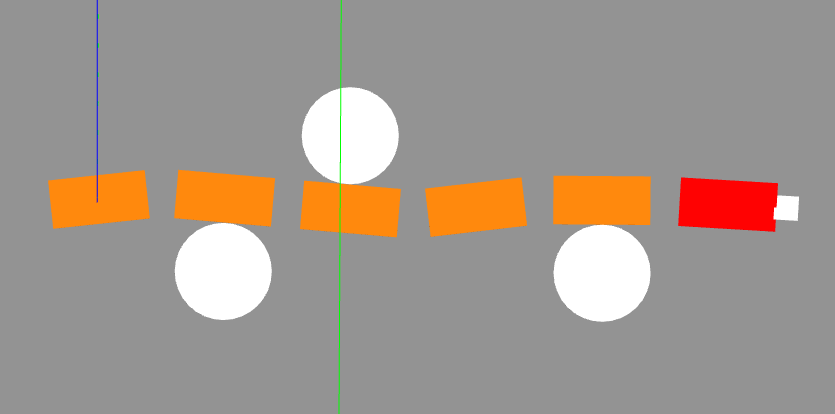
\includegraphics[width=0.6\textwidth]{figures/experiments/initial-gazebo.png}
    \caption{Initial snake robot configuration for dynamic HPFC experiments}
    \label{fig:init-gazebo}
\end{figure}

The control experiments are all based on the dynamic HPFC from \ref{subsec:DHPFC}. The modifications and control structure for the different experiments are presented in the respective sections. All control goals are chosen as simple values to focus the results on the deployed methods. These desired values describe the force against the obstacles and the angle of links in contact with the obstacles. Only a subset of the variables are chosen to be controlled to their desired value for the different experiments. 